\documentclass[12pt]{article}
\usepackage{times} 			% use Times New Roman font

\usepackage[margin=1in]{geometry}   % sets 1 inch margins on all sides
\usepackage{hyperref}               % for URL formatting
\usepackage[pdftex]{graphicx}       % So includegraphics will work
\setlength{\parskip}{1em}           % skip 1em between paragraphs
\usepackage{indentfirst}            % indent the first line of each paragraph
\usepackage{datetime}
\usepackage[small, bf]{caption}
\usepackage{listings}               % for code listings
\usepackage{xcolor}                 % for styling code
\usepackage{multirow}

%New colors defined below
\definecolor{backcolour}{RGB}{246, 246, 246}   % 0xF6, 0xF6, 0xF6
\definecolor{codegreen}{RGB}{16, 124, 2}       % 0x10, 0x7C, 0x02
\definecolor{codepurple}{RGB}{170, 0, 217}     % 0xAA, 0x00, 0xD9
\definecolor{codered}{RGB}{154, 0, 18}         % 0x9A, 0x00, 0x12

%Code listing style named "gcolabstyle" - matches Google Colab
\lstdefinestyle{gcolabstyle}{
  basicstyle=\ttfamily\small,
  backgroundcolor=\color{backcolour},   
  commentstyle=\itshape\color{codegreen},
  keywordstyle=\color{codepurple},
  stringstyle=\color{codered},
  numberstyle=\ttfamily\footnotesize\color{darkgray}, 
  breakatwhitespace=false,         
  breaklines=true,                 
  captionpos=b,                    
  keepspaces=true,                 
  numbers=left,                    
  numbersep=5pt,                  
  showspaces=false,                
  showstringspaces=false,
  showtabs=false,                  
  tabsize=2
}

\lstset{style=gcolabstyle}      %set gcolabstyle code listing

% for fancy page headings
\usepackage{fancyhdr}
\setlength{\headheight}{13.6pt} % to remove fancyhdr warning
\pagestyle{fancy}
\fancyhf{}
\rhead{\small \thepage}
\lhead{\small HW 1, Conner}  % EDIT THIS, REPLACE # with HW number
\chead{\small CS 432, Fall 2020} 

%-------------------------------------------------------------------------
\begin{document}

\begin{centering}
{\large\textbf{HW 1 - Webscience Intro}}\\ % EDIT THIS
                                % REPLACE # with HW num and ADD title
Jacob Conner\\                     % EDIT THIS
September 20, 2020\\                      % EDIT THIS
\end{centering}

%-------------------------------------------------------------------------

% The * after \section just says to not number the sections
\section*{Q1}
Consider the "bow-tie" structure of the web in the Broder et al. paper (http://snap.stanford.edu/class/cs224w-readings/broder00bowtie.pdf) that was described in Week 1.
Now consider the following links (\ref{lst:listNodes}) Draw the resulting graph (either sketch on paper or use another tool) and include an image in your report.)

\begin{lstlisting}[numbers=none, caption=Links, label=lst:listNodes]
A --> B
B --> A
B --> C
C --> D
C --> G
D --> A
D --> H
E --> F
E --> O
F --> G
G --> P
H --> L
J --> N
K --> I
M --> A
N --> L
O --> J
P --> C
\end{lstlisting}

For the above graph, list the nodes (in alphabetical order) that are each of the following categories:
\begin{itemize}
  \item IN:
  \item SCC:
  \item OUT:
  \item Tendrils:
	\begin{itemize}
		\item indicate if the tendril is reachable from IN or can reach OUT
	\end{itemize}
\item Tubes:
	\begin{itemize}
		\item explain how the nodes serve as tubes
	\end{itemize}
\item Disconnected:
\end{itemize}

\subsection*{Answer}

\emph{All figures must have a caption and must be referenced in the text. Example below.}

Figure \ref{fig:bowTieGraph} was created using the \textit{Dia} diagramming tool \cite{dia} and shows the relationships between each node.

\begin{figure}[h]
    \centering
    % trim and clip are used to crop the image, trim=left bottom right top
    % width sets max width, height will be scaled appropriately
    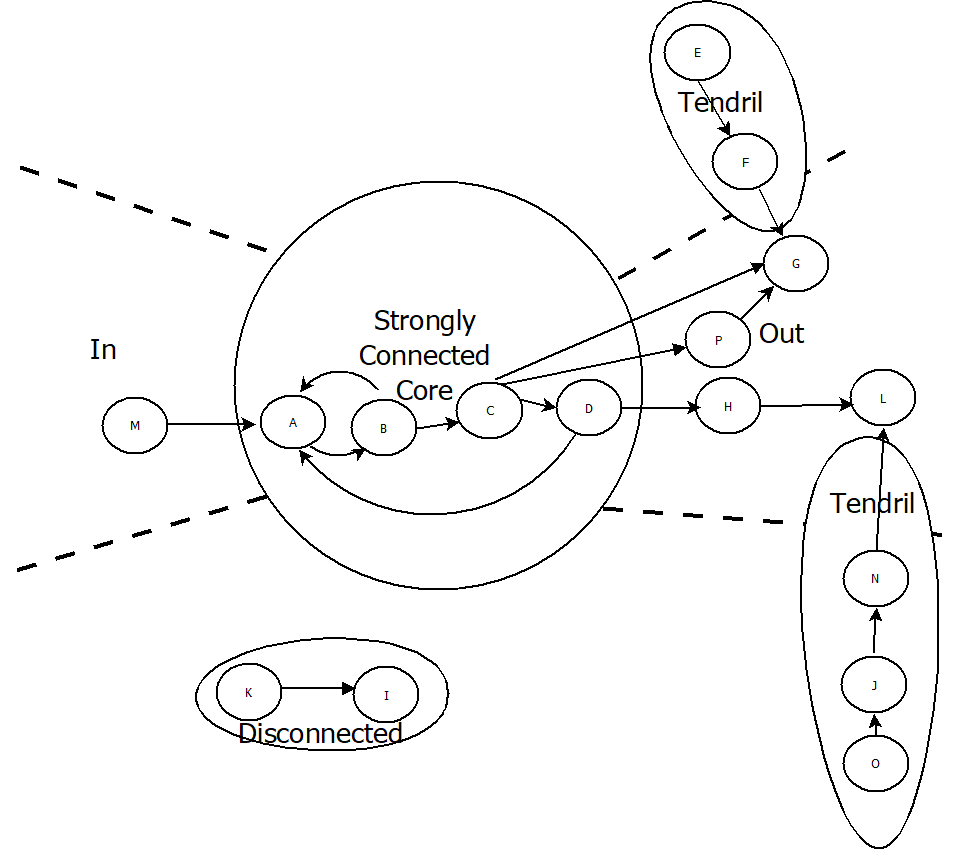
\includegraphics[trim=0 20 10 50, clip, width=\textwidth] {Q1/Q1.png}
    \caption{Bow-Tie Graph representing relationship between nodes}
    \label{fig:bowTieGraph}
\end{figure}

\begin{itemize}
  \item IN: M
  \item SCC: A, B, C, D
  \item OUT: G, H, L,
  \item Tendrils : NONE
	\begin{itemize}
		\item Reaching outward (FROM IN): NONE
		\item: Reaching in (to OUT): E, F, J, N, O
	\end{itemize}
\item Tubes: NONE
\item Disconnected: K, I
\end{itemize}

\subsection*{Discussion}
\emph{You must provide some discussion of every answer. Discuss how you arrived at the answer and the tools you used. Discuss the implications of your answer.}
In this graph, the strongly connected component (SCC)  consists of the sub-graph where all nodes are capable of reaching each other. Table  lists the paths. The in portionn of the graph was detrmined by identifying those nodes that only linked in to another in node or to the SCC. Similarly the OUT nodes were identified by find those nodes that only linked out from another SCC node or to another out node. Tendrils are the groups of nodes that either link out from an IN node or link inward to an OUT node. In this graph, there were not any nodes linking outward from the  IN nodes, but there were three nodes (J, N, O) that reached in to the OUT Node L. Tubes are the nodes that that link between IN and OUT nodes without going through the SCC. Since there were no nodes linking from IN to the OUT nodes, there were no tubes. Then disconnected nodes were the nodes that do not connect to the SCC, IN, OUT are the disconnected nodes. In this graph, there were two disconnected nodes K and I.. Node K can connect to Node I but cannot connect to anything else and Node I serves only as a destination for Node K and does not link to anything else. 

A few interesting observations from this graph is that there are several things that will prevent webcrawlers from discovering all websites. First some nodes are disconnected and are not linked to from any other website. It is simply not possible to uncover these websites by following links. However, even if all nodes were somehow connected, it may be impossible to find websites based on where the webcrawler is searching at from the graph. If I started crawling at the SCC node A, I would be able to find most of the nodes in this graph, but I would never be able to reach node M since it is merely linking to A and A does not link back to M. A webcrawl would also  never be able to uncover any of the tendrils since they link to out nodes, but the out nodes do not link back to them.If by some chance a webcrawler started on an out node then the number of websites that it could uncover would be quite small. 

\begin{table}[h]
\centering
\caption{SCC Links}
\label{tbl:scclinks}
\begin{tabular}{|l|l|l|l|l|}
\hline
\textbf{col} & \textbf{A} & \textbf{B} & \textbf{C} & \textbf{D} \\ \hline \hline
A & X & A,B & A,B,C & A,B,C,D \\ \hline
B & B,A & X & B,C & B,C,D \\ \hline
C & C,D,A & C,D,A,B & X & C,D \\ \hline
D & D,A & D,A,B & D,A,B,C & X \\ \hline
\end{tabular}
\end{table}

\section*{Q2}
Demonstrate that you know how to use curl and are familiar with the available options.



a) In a single curl command, request the URI, show the HTTP response headers, follow any redirects, and change the User-Agent HTTP request field to "CS432/532". Show command you used and the result of your execution on the command line. (Either take a screenshot of your terminal or copy/paste into a code segment.)

b) Then make the same request again, but without showing the HTTP response headers and with saving the HTML output to a file. Show the command you used and the result of your execution on the command line. View that file in a browser and take a screenshot.

c) Finally, load the URI directly from your browser and take a screenshot.

Explain the results you get for each of these steps.
\subsection*{Answer}
a)
\begin{lstlisting}[numbers=none, caption=Command, label=lst:q2ACommand]
curl -i -L -A "CS432/532" http://www.cs.odu.edu/~mweigle/courses/cs532/ua_echo.php
\end{lstlisting}
\begin{lstlisting}[numbers=none, caption=Response, label=lst:q2AResponse]
  % Total    % Received % Xferd  Average Speed   Time    Time     Time  Current
                                 Dload  Upload   Total   Spent    Left  Speed
100   178  100   178    0     0   2282      0 --:--:-- --:--:-- --:--:--  2825
100   114  100   114    0     0    561      0 --:--:-- --:--:-- --:--:--  1461HTTP/1.1 301 Moved Permanently
Server: nginx
Date: Sat, 29 Aug 2020 15:08:24 GMT
Content-Type: text/html
Content-Length: 178
Connection: keep-alive
Location: https://www.cs.odu.edu/~mweigle/courses/cs532/ua_echo.php

HTTP/1.1 200 OK
Server: nginx
Date: Sat, 29 Aug 2020 15:08:24 GMT
Content-Type: text/html; charset=UTF-8
Content-Length: 114
Connection: keep-alive
Vary: Accept-Encoding
X-Powered-By: PHP/5.6.40

<!DOCTYPE html>
<html>
<body>

<br/>USER AGENT ECHO
<br/><br/>
<b>User-Agent:</b> CS432/532<br/>

</body>
</html>
\end{lstlisting}

The curl command is used to make HTTP GET Requests. the -i  or --include flag is used to specify curl to include the headers in the response. The -L or --location flag is used to request the header 
and response for all redirects. The -A or --user-agent flag specifies the User-Agent property in the header that is sends to the string next to it. IN this case the User-Agent sent is "CS432/5432".
Then the last part of the curl command is the URI(s) for the webserver(s) that we are making a HTTP GET request to /cite{curlManPage}.

b)
\begin{lstlisting}[numbers=none, caption=Command, label=lst:q2BCommand]
curl -o response.html -L -A "CS432/532" http://www.cs.odu.edu/~mweigle/courses/cs532/ua_echo.php
\end{lstlisting}

\lstinputlisting[language=HTML, caption=response.html, label=lst:responseHtml]{Q2/response.html}
\begin{figure}[h]
    \centering
    % trim and clip are used to crop the image, trim=left bottom right top
    % width sets max width, height will be scaled appropriately
    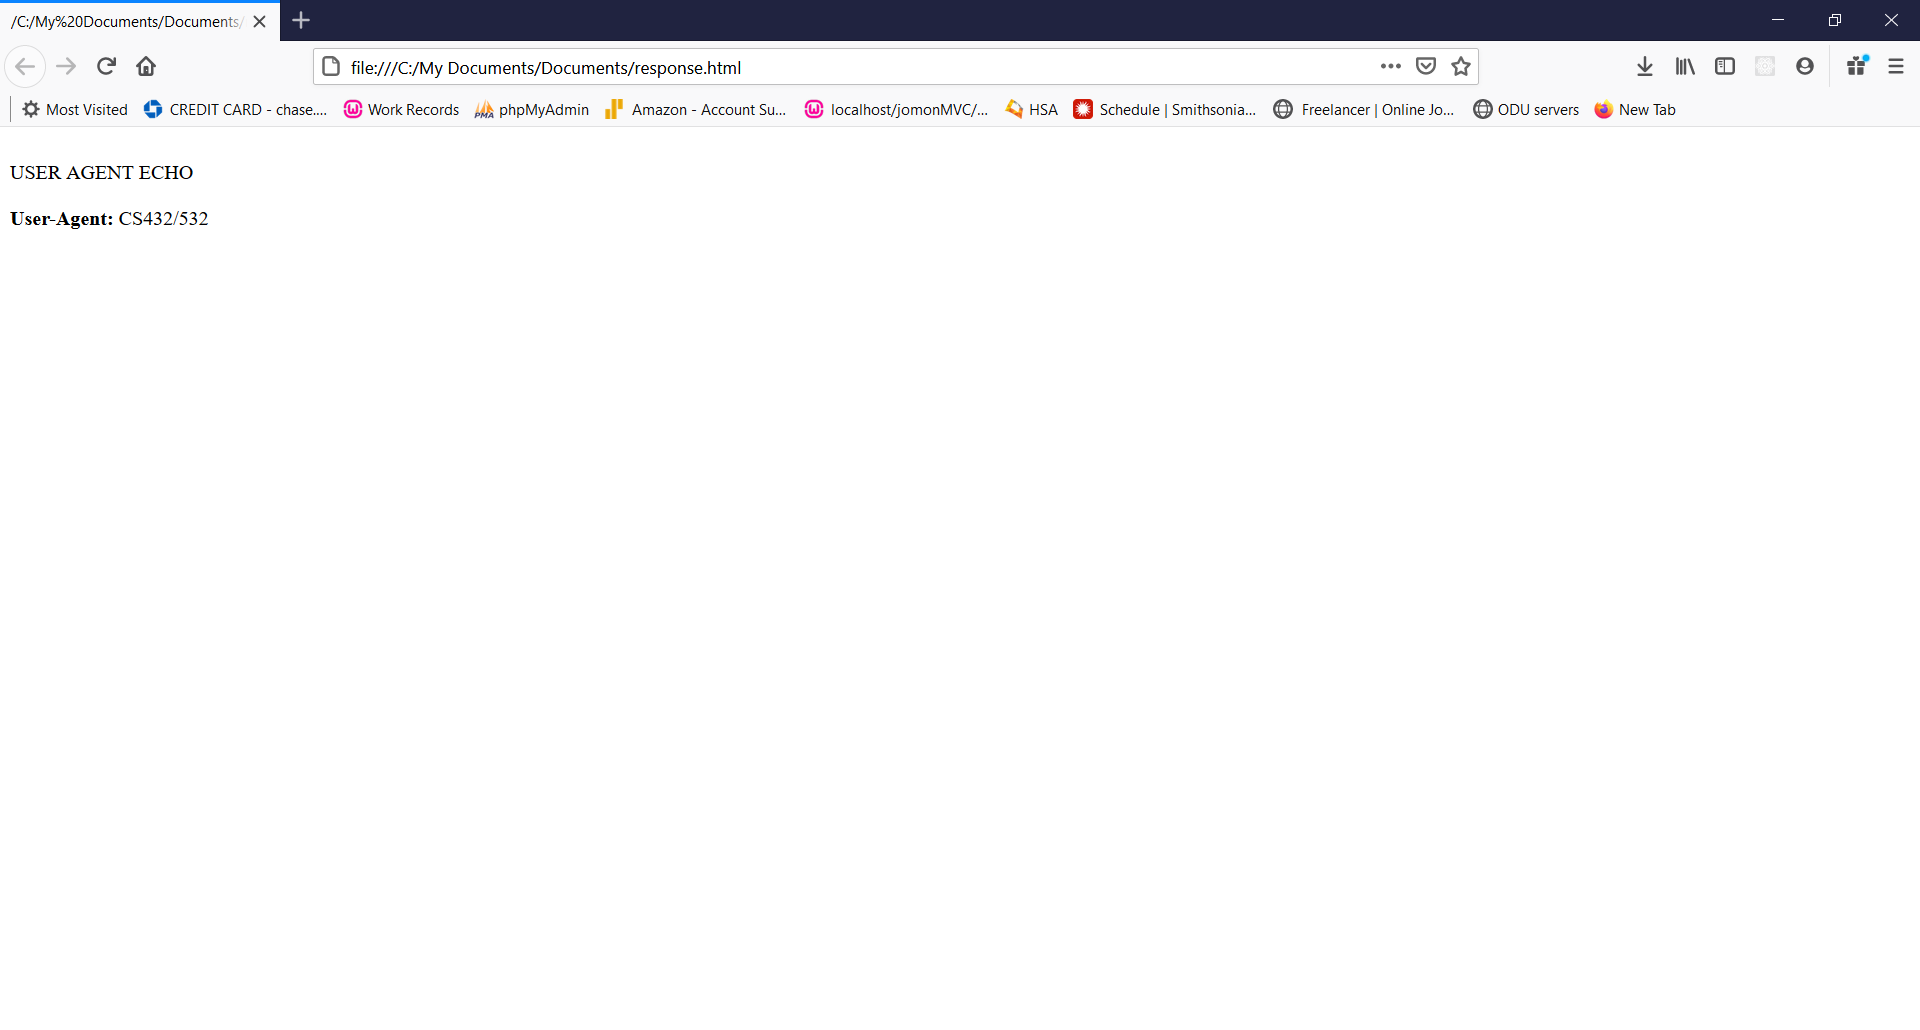
\includegraphics[trim=0 20 10 50, clip, width=\textwidth] {Q2/Q2b_Screenshot.png}
    \caption{Response 2}
    \label{fig:q2BResponse}
\end{figure}

This command is similar to the previous command in part a. However since we do not need the header information, the -i --include flag has been omitted. I have also added the -o output flag to copy the resulting
response from the server into the file response.html. /ref{lst:responseHtml} shows the result output from the HTTP request. The response.html file is a fairly simple html file with a body tag enclosing one set of bold tags surrounding the words User-Agent, and  the value of our User-Agent property (CS432/532) in the GET request header. The browser representation of the response is displayed in \ref{fig:q2BResponse}
c)
\begin{figure}[h]
    \centering
    % trim and clip are used to crop the image, trim=left bottom right top
    % width sets max width, height will be scaled appropriately
    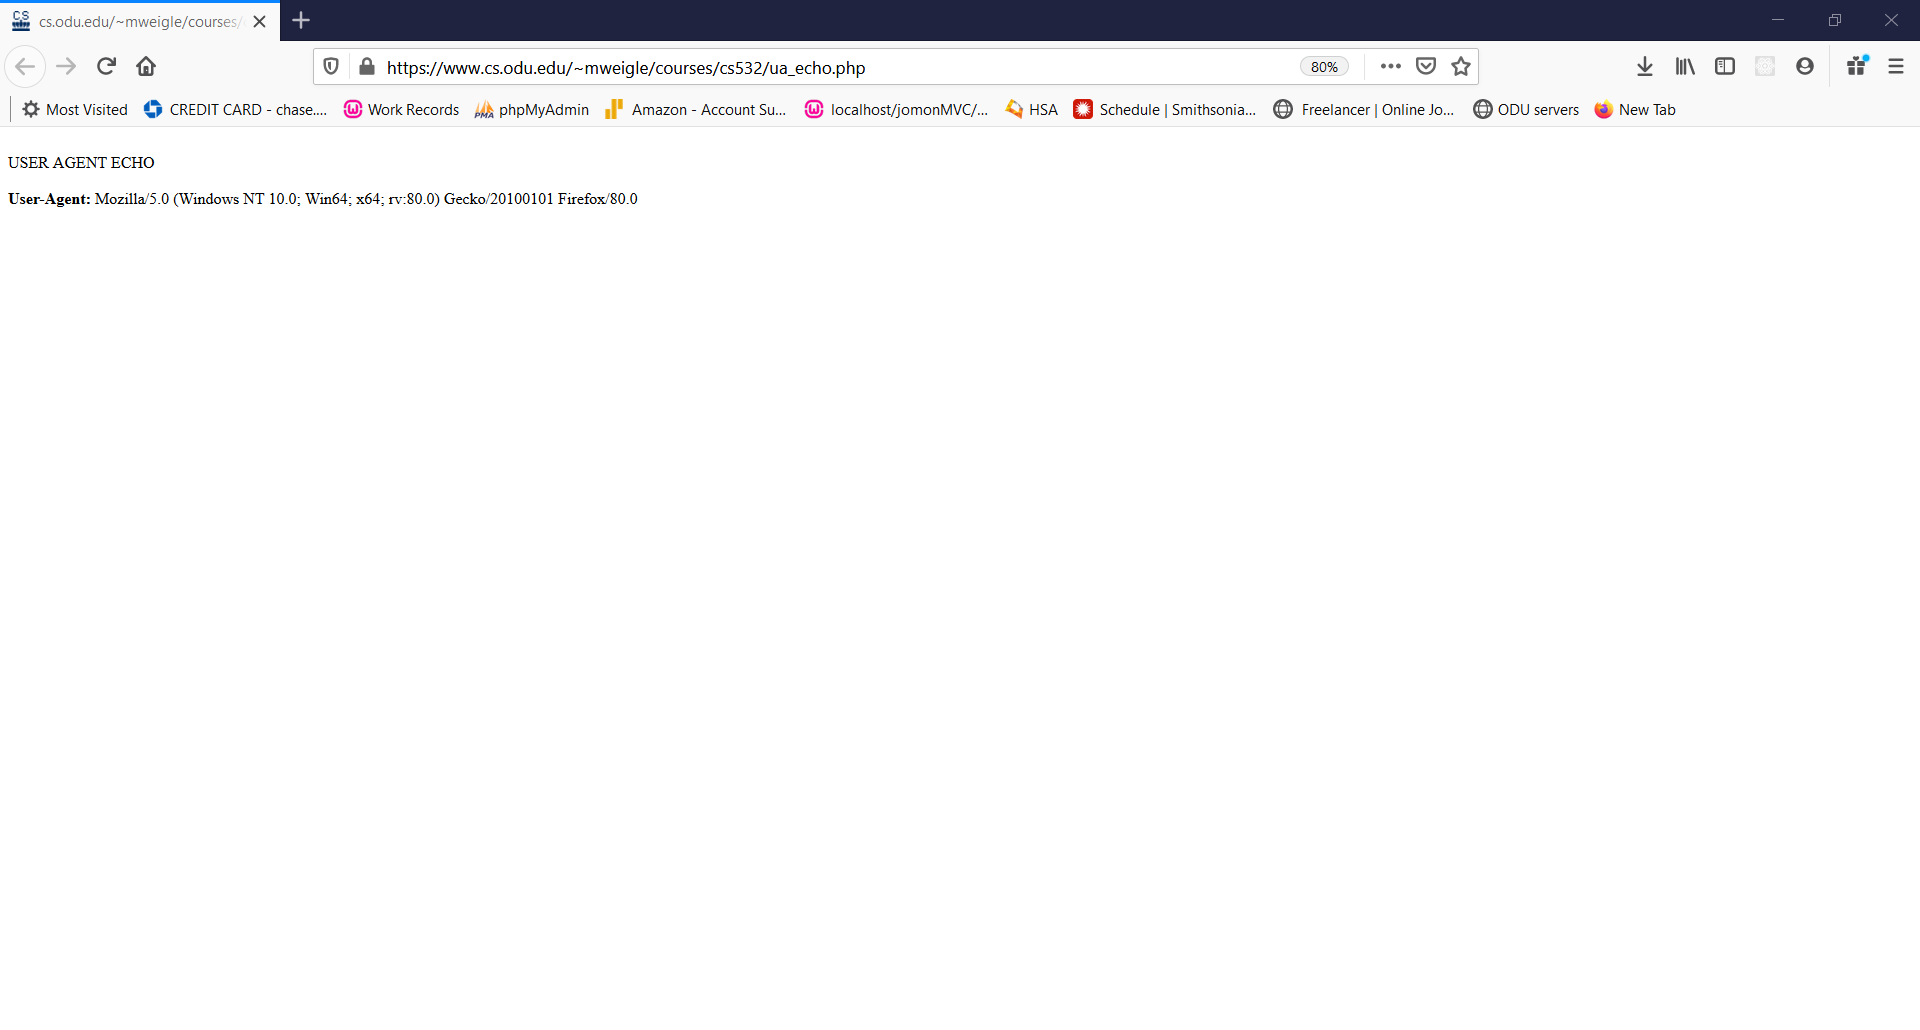
\includegraphics[trim=0 20 10 50, clip, width=\textwidth] {Q2/Q2c_Screenshot.png}
    \caption{Response 3}
    \label{fig:q2CResponse}
\end{figure}

If a browser navigates to https://www.cs.odu.edu/~mweigle/courses/cs532/ua\_echo.php, the browser sends the GET HTTP request in the background and receives the Response and creates a representation of
 the response which will look similar to /ref{fig:g2CResponse}. It looks very similar to the previous response.html retrieved from the curl command, but in the browser the User-Agent shows a different string. One
the computer I am currently using, I am running Windows 10 64-bit and running Firefox, so the Browser uses that information to send a string to the User-Agent in the GET request to help the webserver identify
how I am accessing this page. If I were to use a different browser such as Chrome or if I ran firefox on a linux distribution, I would get a different string. On every GET Request submitted by the browser, this same
User-Agent string is submitted.

\subsection*{Discussion}
In this section, different types of GET Requests were examined. In the first two questions, the GET HTTP Request was created using the curl command and the headers had to be specified using User-Agent. Then
in the last question, a browser was used to issue a GET request for https://www.cs.odu.edu/~mweigle/courses/cs532/ua\_echo.php and the browser automatically created a User-Agent string for the header. One interesting
takeaway from this exercise is that a webserver can very easily identify if a browser or another program is issuing a GET request because the browser sends a User-Agent string and other programs do not by default. 


\section*{Q3}
Write a Python program to find links to PDFs in a webpage.

Your program must do the following:
\begin{itemize}
    \item take the URI of a webpage as a command-line argument
    \item extract all the links from the page
    \item for each link, use the Content-Type HTTP response header to determine if the link references a PDF file
    \item for all links that reference a PDF file, print the original URI (found in the source of the original HTML), the final URI (after any redirects), and the number of bytes in the PDF file. (Hint: Content-Length HTTP response header)
\end{itemize}
Show that the program works on 3 different URIs, one of which must be https://www.cs.odu.edu/~mweigle/courses/cs532/pdfs.html
Here is a snippet of the expected operation:

\begin{lstlisting}[numbers=none, caption=Expected Output, label=lst:q3ExpectedOutput]
% python3 findPDFs.py https://www.cs.odu.edu/~mweigle/courses/cs532/pdfs.html

URI: http://www.cs.odu.edu/~mln/pubs/ht-2015/hypertext-2015-temporal-violations.pdf
Final URI: https://www.cs.odu.edu/~mln/pubs/ht-2015/hypertext-2015-temporal-violations.pdf
Content Length: 2,184,076 bytes

URI: http://www.cs.odu.edu/~mln/pubs/tpdl-2015/tpdl-2015-annotations.pdf
Final URI: https://www.cs.odu.edu/~mln/pubs/tpdl-2015/tpdl-2015-annotations.pdf
Content Length: 622,981 bytes
\end{lstlisting}

\subsection*{Answer}
Listing \ref{lst:findPDFs} is the imported code I used to scrape pdf files from webpages.

\lstinputlisting[language=Python, caption=FindPDFs.py, label=lst:findPDFs]{Q3/findPDFs.py}

Below I have provided screenshots of various sample output from the findPDFs.py scraper. 
\ref{fig:q3ResponseWeigle} is the output I received after running the findPDFs.py scraper on https://www.cs.odu.edu/ mweigle/courses/cs532/pdfs.html 
\begin{figure}[h]
    \centering
    % trim and clip are used to crop the image, trim=left bottom right top
    % width sets max width, height will be scaled appropriately
    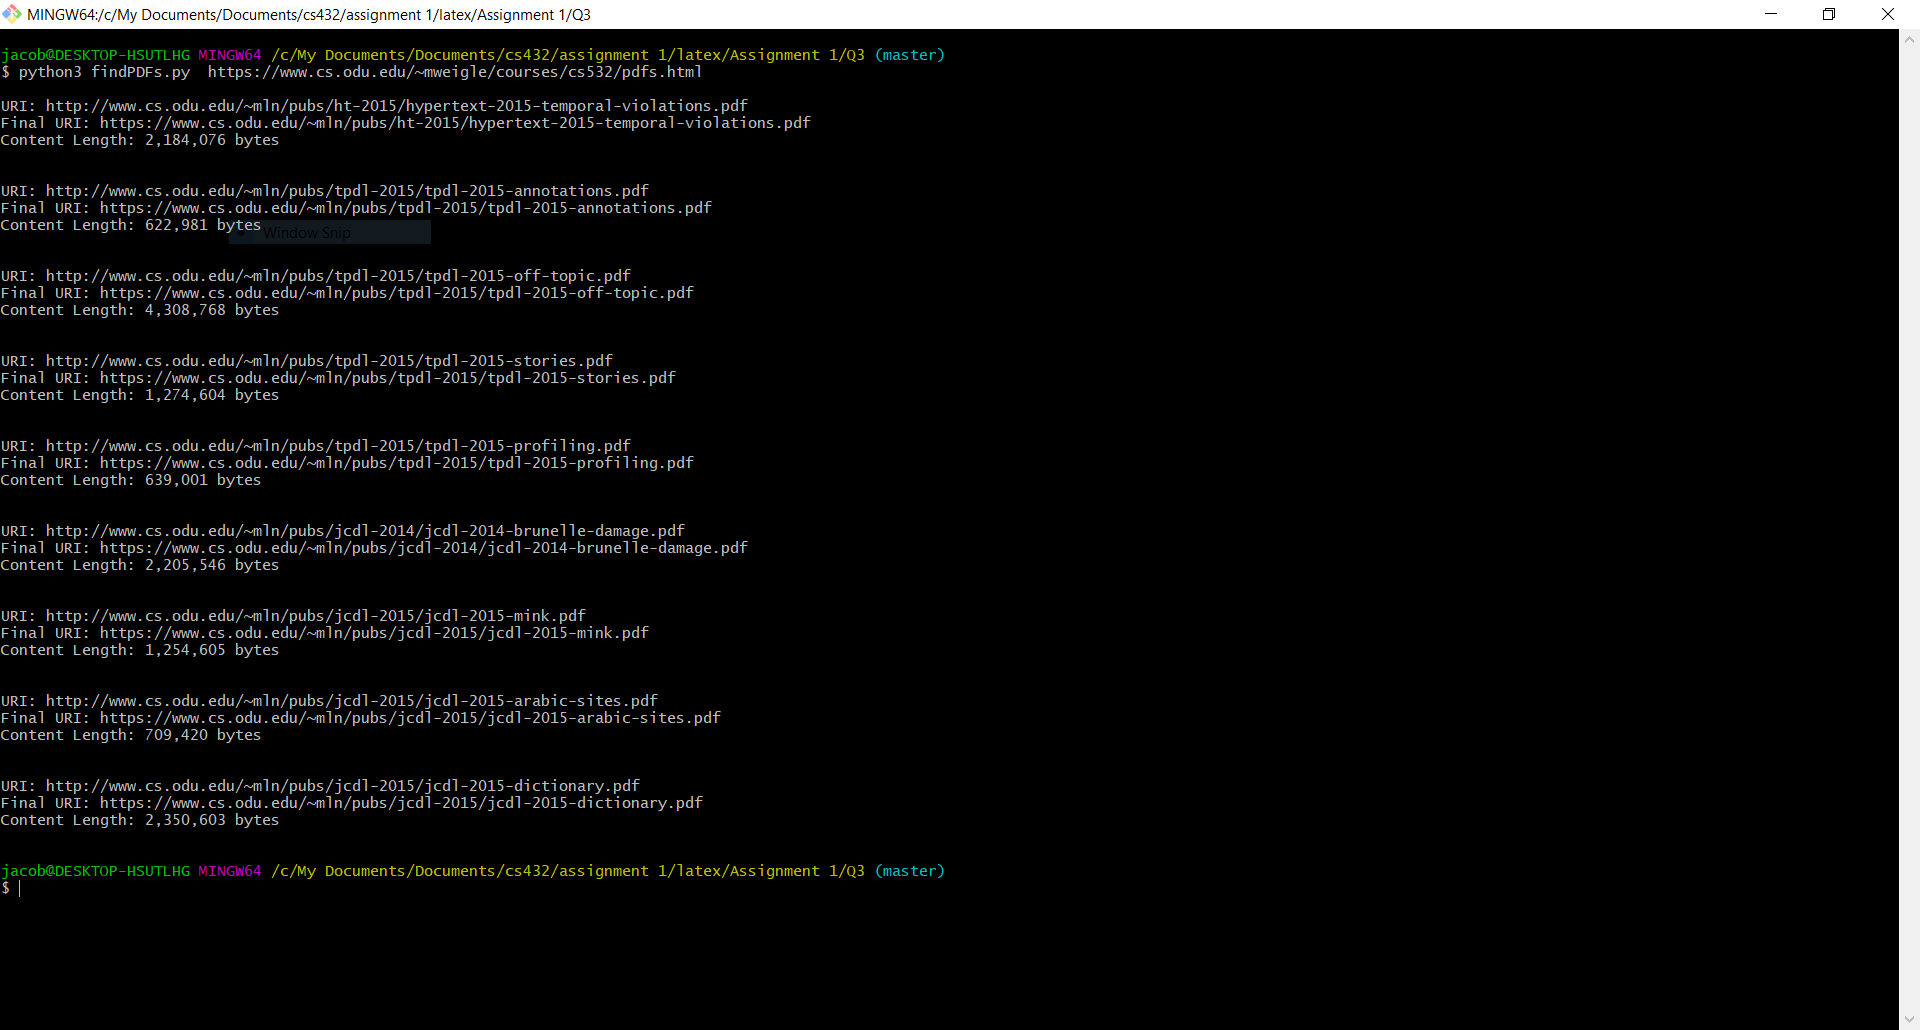
\includegraphics[trim=0 20 10 50, clip, width=\textwidth] {Q3/q3_weiglePdfs.png}
    \caption{findPDFs.py results for https://www.cs.odu.edu/ mwei-
gle/courses/cs532/pdfs.html}
    \label{fig:q3ResponseWeigle}
\end{figure}

\ref{fig:q3ResponseUbuntu} is the output I received after running the findPDFs.py scraper on the Ubuntu manual page (https://help.ubuntu.com/)
\begin{figure}[h]
    \centering
    % trim and clip are used to crop the image, trim=left bottom right top
    % width sets max width, height will be scaled appropriately
    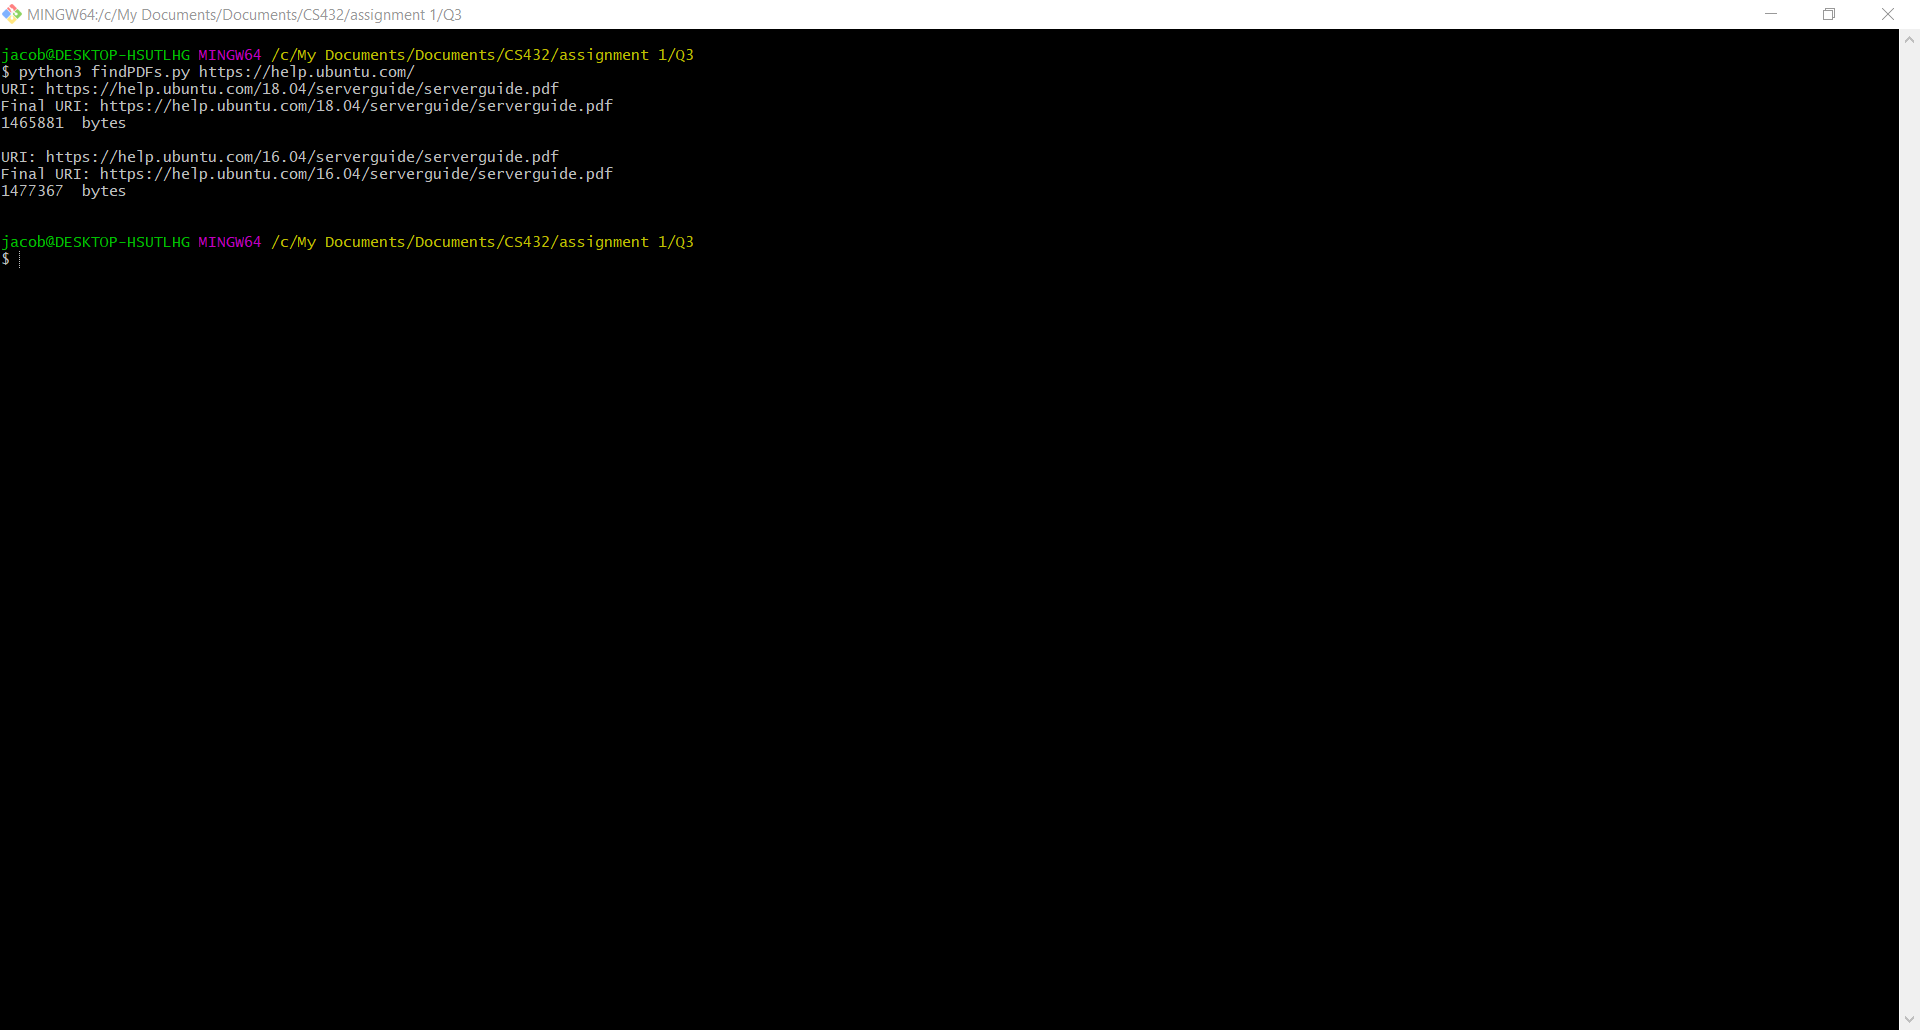
\includegraphics[trim=0 20 10 50, clip, width=\textwidth] {Q3/q3_ubuntuHelp.png}
    \caption{findPDFs.py results for https://help.ubuntu.com/}
    \label{fig:q3ResponseUbuntu}
\end{figure}

\ref{fig:q3ResponsecranR_1} and \ref{fig:q3ResponsecranR_2} are screenshots of the output I received after running the findPDFs.py scraper on the CRAN-R R programming manuals page (https://cran.r-project.org/manuals.html)
\begin{figure}[h]
    \centering
    % trim and clip are used to crop the image, trim=left bottom right top
    % width sets max width, height will be scaled appropriately
    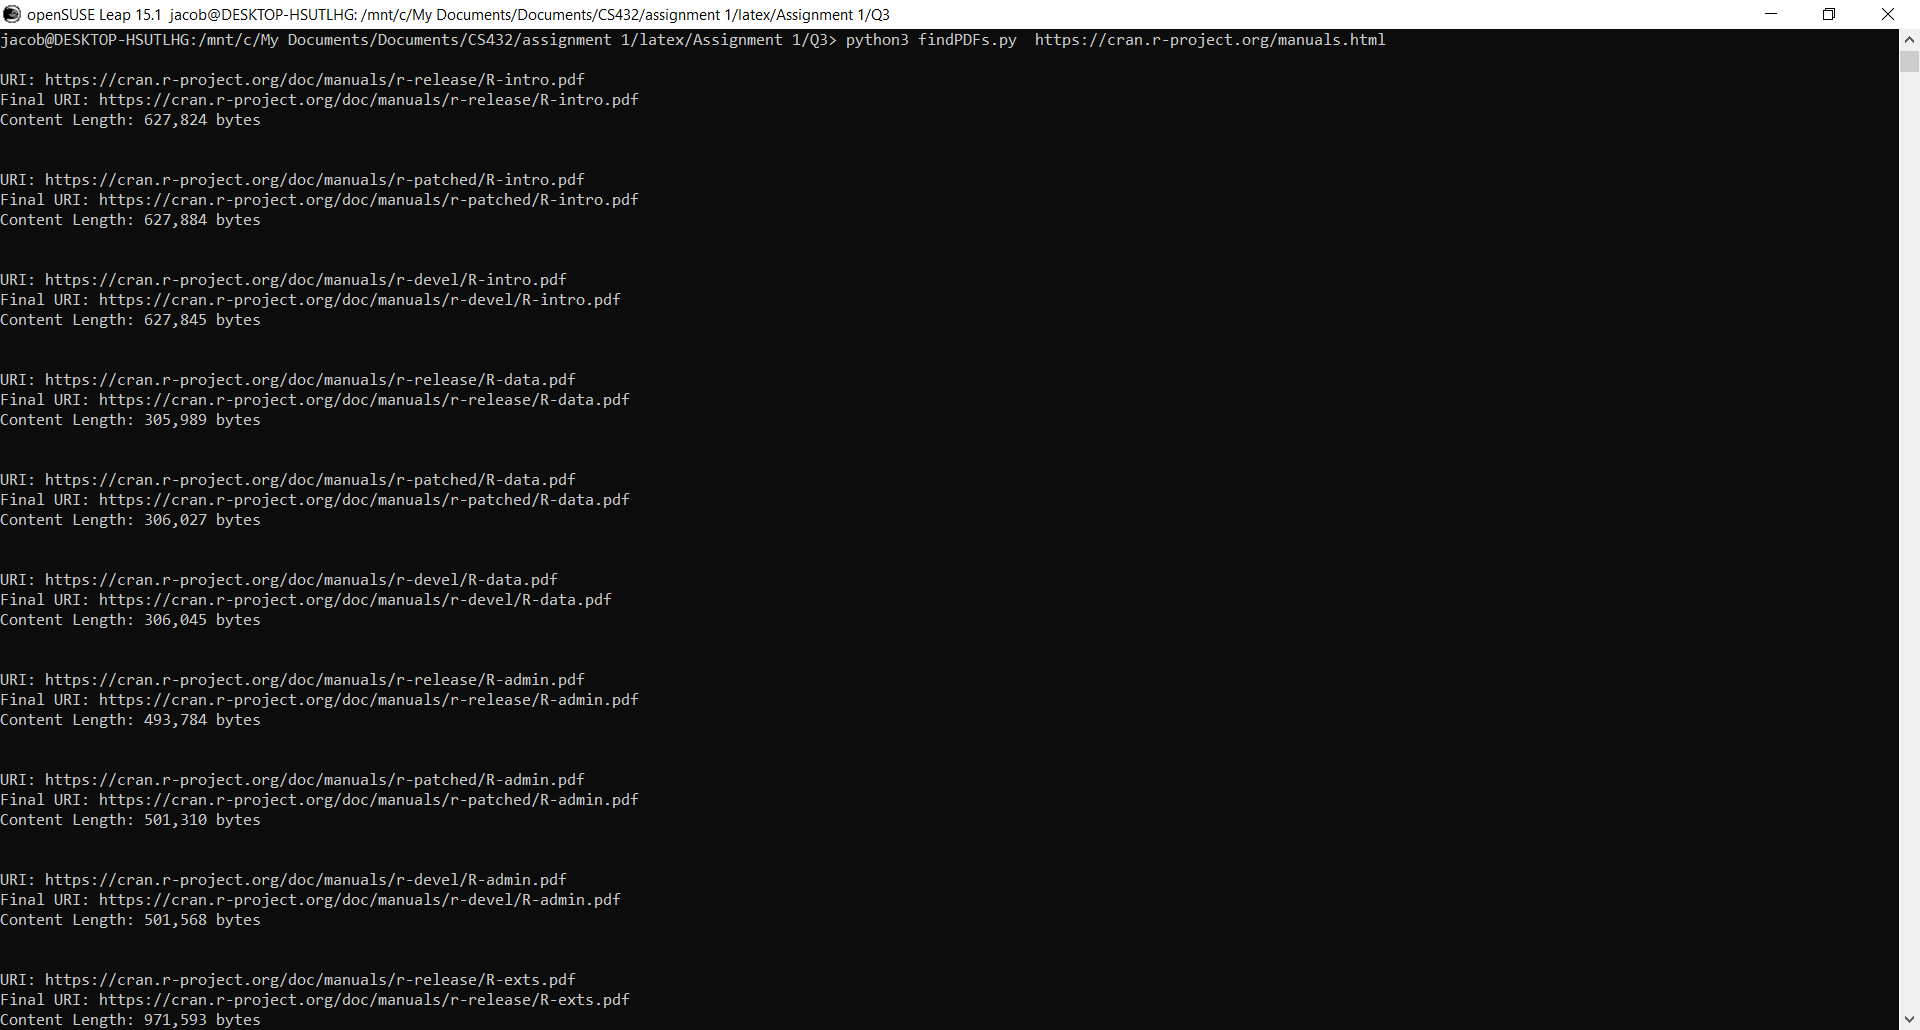
\includegraphics[trim=0 20 10 50, clip, width=\textwidth] {Q3/q3_cranRManuals.png}
    \caption{findPDFs.py results for https://cran.r-project.org/manuals.html}
    \label{fig:q3ResponsecranR_1}
\end{figure}


\begin{figure}[h]
    \centering
    % trim and clip are used to crop the image, trim=left bottom right top
    % width sets max width, height will be scaled appropriately
    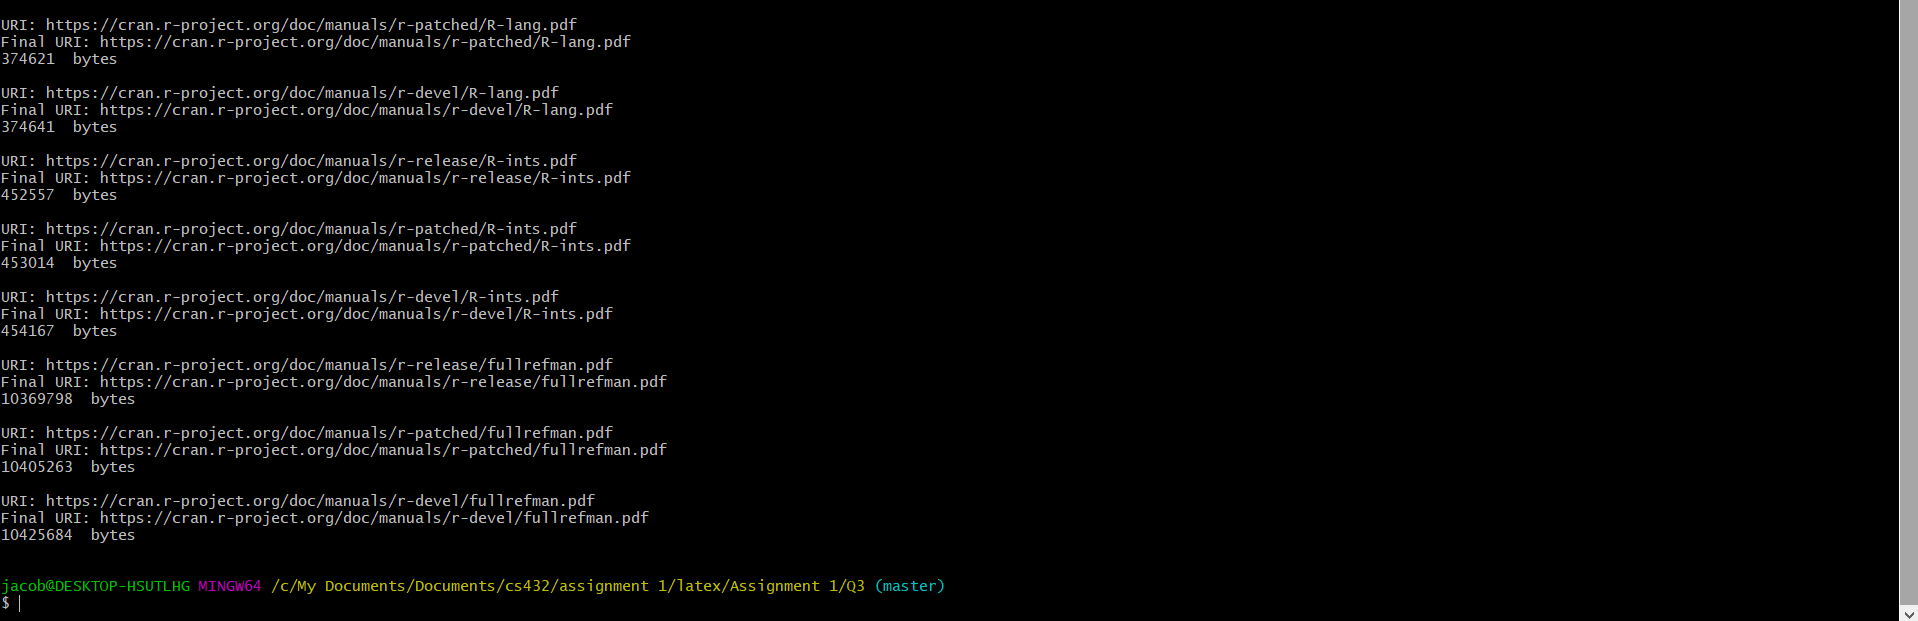
\includegraphics[trim=0 20 10 50, clip, width=\textwidth] {Q3/q3_cranRManuals2.png}
    \caption{findPDFs.py results for https://cran.r-project.org/manuals.html}
    \label{fig:q3ResponsecranR_2}
\end{figure}

\ref{fig:q3ResponseSEAA_1} and \ref{ig:q3ResponseSEAA_1} are screenshots of the output I received after running the findPDFs.py scraper on the Society of East Asian Archaeology's 2018 bulletin page (https://seaa-web.org/publications/bseaa/bulletin-society-east-asian-archaeology)
\begin{figure}[h]
    \centering
    % trim and clip are used to crop the image, trim=left bottom right top
    % width sets max width, height will be scaled appropriately
    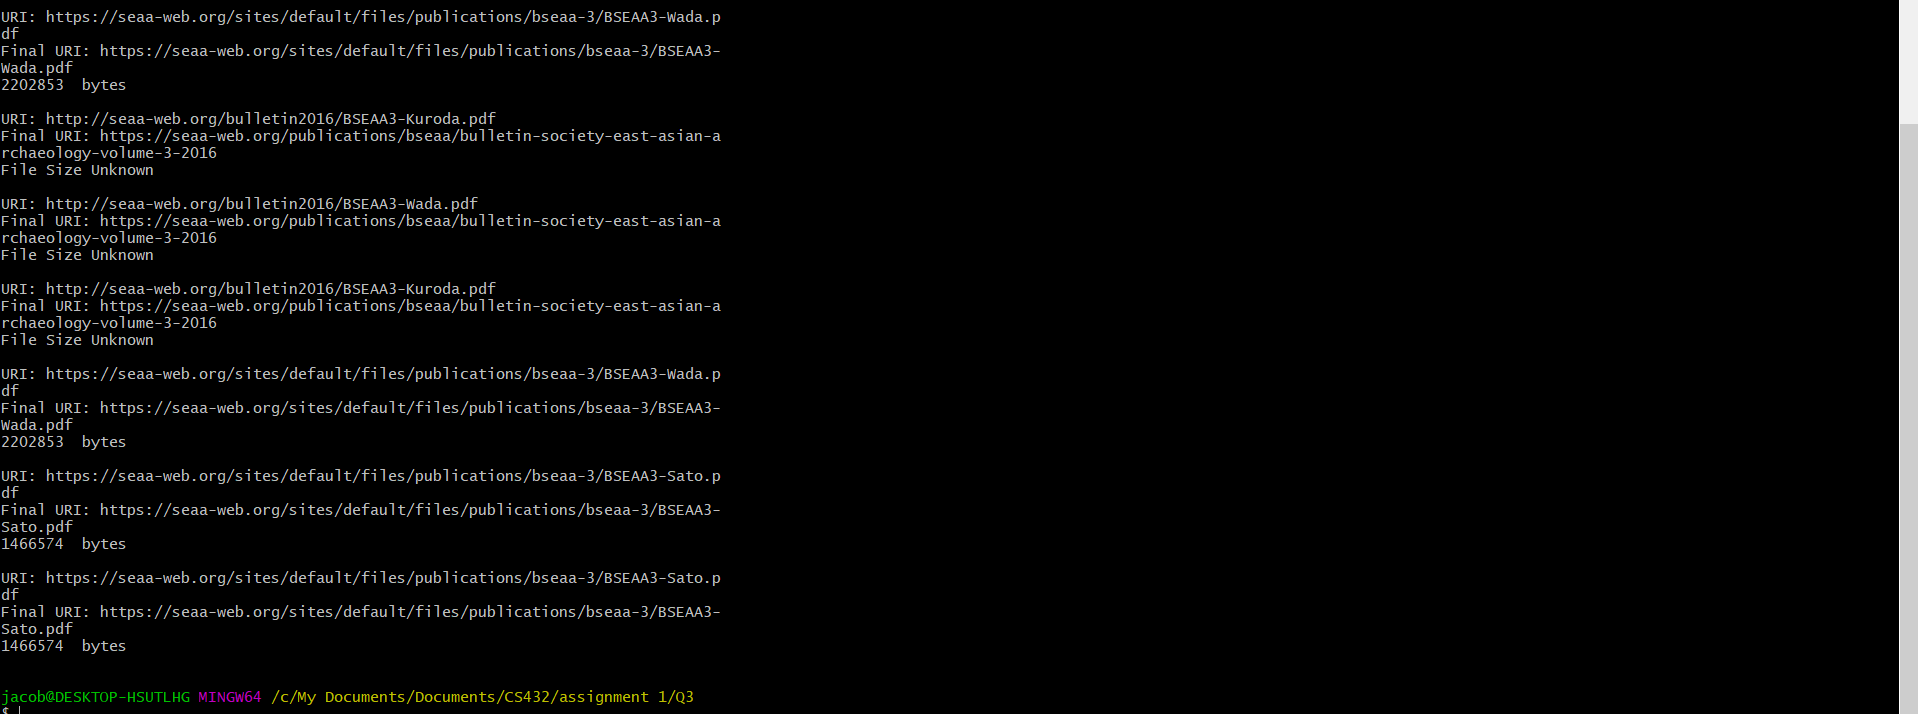
\includegraphics[trim=0 20 10 50, clip, width=\textwidth] {Q3/q3-seaaBulletin2016-2.png}
    \caption{findPDFs.py results for https://seaa-web.org/publications/bseaa/bulletin-society-east-asian-archaeology}
    \label{fig:q3ResponseSEAA_1}
\end{figure}


\begin{figure}[h]
    \centering
    % trim and clip are used to crop the image, trim=left bottom right top
    % width sets max width, height will be scaled appropriately
    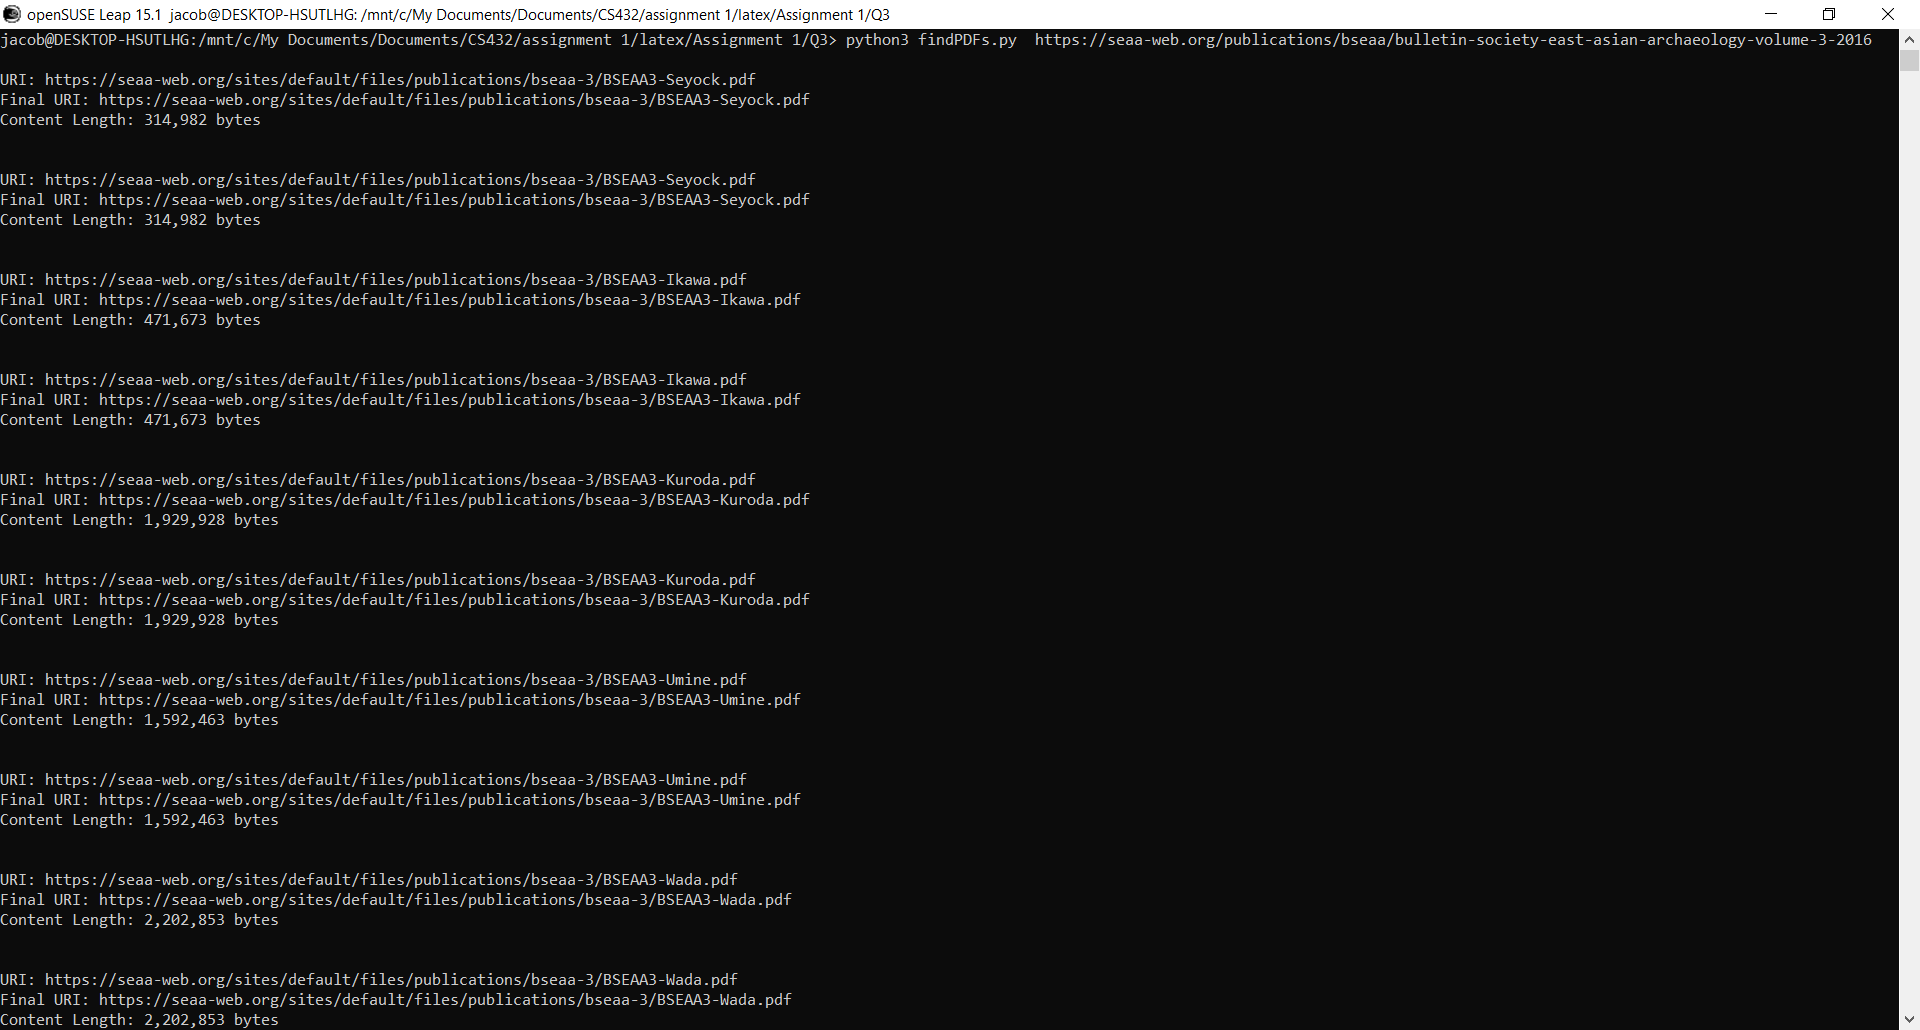
\includegraphics[trim=0 20 10 50, clip, width=\textwidth] {Q3/q3-seaaBulletin2016.png}
    \caption{findPDFs.py results for https://seaa-web.org/publications/bseaa/bulletin-society-east-asian-archaeology}
    \label{fig:q3ResponseSEAA_2}
\end{figure}


\subsection*{Discussion}

The code above generates a console program that accepts a url parameter from the user . If no url is provided, the program exits. Next a HTTP GET request is made to the URL sent with a  User-Agent header to allow the code to run on more webservers.
Once the response from the webserver that the URL points to is received, the resulting text from the response is parsed using the BeautifulSoup library to retrieve all of the anchor ('a') tags in the document. Then every anchor's 'href' attribute is tested to see if it is an absolute path and if the url is a relative path then it is converted to be an absolute path. After the link is in the correct form, it is checked to see if it is a pdf and another HTTP Request is made for each URL. The resulting response from the HTTP request is used to print the URI, Final URI and file size output to the console. 

In order to accomplish task, I have created a main function with 6 other functions. The The main function begins with retrieving the url  from the user input. THe user input is handled using the checkForArgumentsfunction. This function uses Python's built in sys library's argv function to get the first command from the user. A conditional is used to check if the the argv variable exists and if not, it exits the program. This function only cares that there is a second parameter after the findPDFs.py command and does not evaluate if it is a valid url or not.

The validateRequest function validates the user's url and any other uri, we provide it. Since some webservers do not like webscrapers and will reject their GET requests, the validateRequest function begins with building a header and generates a User\_Agent string to mimic a browser's User-Agent string using a modified version of the GET\_UA function.\cite{randomizeUserAgent}. TheThe GET\_UA function is simply a list of User Agents that I created using 5 different browserson Windows 10 (Firefox, Chrome, Eduge, Opera, and Internet Explorer) and obtained by visiting whatismyip.com \cite{whatIsMyIp} to get the User Agent. Then this function use Python's built in random library to pick one of these User\_Agent strings at random. The validateRequest function uses the resulting User\_Agent to build a header. A try catch block is used to try a HTTP GET request using the requests library. If a response is received, the validateRequest function returns it.
If it fails, an Exception is generated and the function returns None. 

After retrieving the response, the /emph{main} function uses the BeautifulSoup library to parse the HTM to retrieve all anchor tags. There are numerous HTML parsers available including python's built in HTMLParser library, but in order to make use
of that library to get all of the anchor tags, a subclass of HTMLParser has to be created and various methods have to be overriden. the BeautifulSoup library is able to do this with a single line that initializes the BeautifulSoup  object with
the HTTP GET request's response's text and then calls the FindAll method to retrieve all anchor tags. So BeautifulSoup was used in this case for the sake of conciseness.  BeautifulSoup returns a list-like object that is iterated through using a for loop in order to check each anchor tag's 'href' attribute. 

Now that I have a list of links, I need to format them so they are ready for the response requests. The first modification made is ensure the url is an absolute path. Since many websites make use of  relative URLs to make the code easier to port between testing and production environments, I have modified an absolutePath function \cite{stackOverflowRelativePath} to check if a url starts with "http://www" or "http://www" and if not, the function assumes the link found was a relative url. In order to convert the relative url to an absolute url, I made use of python's urllib library to combine the two urls using the parse.urljoin method. 

Next the The /emph{checkIfPDFRegEx} function is used to check if the link is a pdf. This function uses the re (regular expression) libary to check if a url ends in '.pdf' and if it ends in .pdf, the function assumes the link is a pdf. This will find all pdfs as long as the file has the extension. I found a website \cite{anthropologicalScienceWebsite} that has several PDFs that cannot be retrieved by this due to not having the .pdf extension. An alternative approach to checking for PDFs is to make a GET or HEAD request using the Request library. The resulting response has a headers method that can be called that may contain the property Content-Type. If the property exists, you can check if it is is application/pdf and if so, the link must be a pdf. Unfortunately, the Content-Type property does not always exist. Since thiis approaach does not always work and results in numerous GET or HEAD requests that could result in my webscraper being blocked by the webserver,  I found the Header approach to identify pdfs to be less desirable than the regular expression approach. After verifying the url is a pdf link, the checkIfPDFRegEx function calls the validateRequest function to generate a new GET request and returns the response. If a link is not a PDF, then the function returns None.

The main function ends by calling a the printResult function on all of the responses returned from checkIfPDFRegEx. This function displays the original URI, the final URI (after any redirects) and the size of the pdf file. The URI is created using the original link url (after converting to an absolute path). The final URI is obtained using the GET Request response's url property. The Request library by default will set the url to the final redirect unless the GET Request is sent with an additional argument of allow-redirects=False. If allow-redirects is set to false, then GET requests would have to be made on the resulting response.url until the response.status\_code is no longer 300, 301, 302, 303, 307, or 308. This is quite inefficient and the more HTTP requests to a server in a short period of time, increases the likleihood of being the server blocking the webscraper. Instead, a normal GET request using the requests library can be used and the url property of the response is the final URI after any redirects. If a history of redirects is needed, the history property of the response can be looped through to get all URIs inbetween \cite{stackOverflowRedirects}. The file size of the PDF is found using the 'Content-length'  found in the response's header.  Since header properties can be absent on certain sites, I have made use of a loop to check if it exists, prior to displying the file size to avoid an exception. I rand into this issue when running the program on the Soceity for East Asian Archaeology's site  \cite{bulletin2016SEAA}. Technically everything used in the printResults  can be used using a HEAD Request, however many webservers in an attempt to avoid scrapers do not allow HEAD requests, so a GET request was used. Once all links to pdfs have been displayed, the program ends. 

This code is a fairly decent general purpose webscraping tool for pdfs on most web servers. However I found a few limitations. Some web servers will generate the "'Unable to receive response from  javascript:void(0)". For example I attempted to run the code on Google Scholar search results for Jomon (a prehistoric culture in Japan) \cite{googleScholarJomon} and the program generated this exception. In cases like this, Google's server has blocked my webscraper from running the GET Requests because it is able to identify this is a scraper and not a regular browser. On clever servers like this, I can't make the requests library work and a headless browser approach using a library like Selenium would have to be used. Another limitation I came across and was suprised to see was that some web servers will load files without the file extension. This again is hard to identify. The only ways around this is to check the content-type in the header if it is available or to tailor your scraper to a single website. Websites with lots of pds tend to follow patterns for CSS formatting nd javascript purposes, so it is possible all anchor tags linking to pdfs may be stored uner a div with a unique class. In cases like these a specialized approach to PDF scraping must be used. 

\bibliographystyle{unsrt}
\bibliography{references}


\end{document}

